\section{Labelling} 
\subsection{Label for a point} 
\hypertarget{tlp}{}
It is possible to add several labels at the same point by using this macro several times.  

\begin{NewMacroBox}{tkzLabelPoint}{\oarg{local options}\parg{point}\var{label}}%
\begin{tabular}{lll}%
arguments &  example  &                  \\ 
\midrule
\TAline{point}{\tkzcname{tkzLabelPoint(A)\{\$A\_1\$\}}}{}
options  & default & definition\\
\midrule
\TOline{TikZ options}{}{colour, position etc.}
\bottomrule
\end{tabular}

\medskip
Optionally, we can use any style of \TIKZ, especially placement with above, right, dots...
\end{NewMacroBox}

\subsubsection{Example with \tkzcname{tkzLabelPoint}} 
\begin{tkzexample}[latex=7cm,small]  
\begin{tikzpicture}
  \tkzDefPoint(0,0){A}
  \tkzDefPoint(4,0){B}
  \tkzDefPoint(0,3){C}
  \tkzDrawSegments(A,B B,C C,A)
  \tkzDrawPoints(A,B,C)
  \tkzLabelPoint[left,red](A){$A$}
  \tkzLabelPoint[right,blue](B){$B$}
  \tkzLabelPoint[above,purple](C){$C$}  
\end{tikzpicture} 
\end{tkzexample} 

\subsubsection{Label and reference}
 The reference of a point is the object that allows to use the point, the label is the name of the point that will be displayed.
 
\begin{tkzexample}[latex=6cm,small]
 \begin{tikzpicture}
    \tkzDefPoint(2,0){A} 
    \tkzDrawPoint(A)
    \tkzLabelPoint[above](A){$A_1$}  
  \end{tikzpicture}
 \end{tkzexample}
 
\subsection{Add labels to points \tkzcname{tkzLabelPoints}}
It is possible to place several labels quickly when the point references are identical to the labels and when the labels are placed in the same way in relation to the points. By default, \tkzname{below right} is chosen.
\hypertarget{tlps}{}  

\begin{NewMacroBox}{tkzLabelPoints}{\oarg{local options}\parg{$A_1,A_2,...$}}%
\begin{tabular}{lll}
arguments &  example & result                 \\ 
\midrule
\TAline{list of points}{\tkzcname{tkzLabelPoints(A,B,C)}}{Display of $A$, $B$ and $C$}
\bottomrule
\end{tabular}

\medskip
This macro reduces the number of lines of code, but it is not obvious that all points need the same label positioning.
\end{NewMacroBox}

\subsubsection{Example with \tkzcname{tkzLabelPoints}}   
\begin{tkzexample}[latex = 6cm,small]  
\begin{tikzpicture}
  \tkzDefPoint(2,3){A}
  \tkzDefShiftPoint[A](30:2){B}
  \tkzDefShiftPoint[A](30:5){C}
  \tkzDrawPoints(A,B,C)
  \tkzLabelPoints(A,B,C) 
\end{tikzpicture} 
\end{tkzexample}
%<--------------------------------------------------------------------------->
%                       tkzAutoLabelPoints
%<--------------------------------------------------------------------------->
\subsection{Automatic position of labels \tkzcname{tkzAutoLabelPoints}}
The label of a point is placed in a direction defined by a center and a point \tkzname{center}. The distance to the point is determined by a percentage of the distance between the center and the point. This percentage is given by \tkzname{dist}.
\begin{NewMacroBox}{tkzLabelPoints}{\oarg{local options}\parg{$A_1,A_2,...$}}%
\begin{tabular}{lll}
arguments &  example & result                 \\ 
\midrule
\TAline{list of points}{\tkzcname{tkzLabelPoint(A,B,C)}}{Display of $A$, $B$ and $C$}
\end{tabular}
\end{NewMacroBox}

\subsubsection{Label for points with \tkzcname{tkzAutoLabelPoints}} 
Here the points are positioned relative to the center of gravity of $A,B,C \text{ and } O$.
\begin{tkzexample}[latex=4cm,small]
\begin{tikzpicture}[scale=1]
 \tkzDefPoint(2,1){O}
 \tkzDefRandPointOn[circle=center O radius 1.5]\tkzGetPoint{A}
 \tkzDefPointBy[rotation=center O angle 100](A)\tkzGetPoint{C}
 \tkzDefPointBy[rotation=center O angle 78](A)\tkzGetPoint{B}
 \tkzDrawCircle(O,A) 
 \tkzDrawPoints(O,A,B,C) 
 \tkzDrawSegments(C,B B,A A,O O,C)
 \tkzDefTriangleCenter[centroid](A,B,C) \tkzGetPoint{O}
 \tkzDrawPoint(tkzPointResult)
 \tkzLabelPoints(O,A,C,B)
\end{tikzpicture}
\end{tkzexample}

\section{Label for a segment} 
\hypertarget{tls}{}  
\begin{NewMacroBox}{tkzLabelSegment}{\oarg{local options}\parg{pt1,pt2}\marg{label}}
This macro allows you to place a label along a segment or a line. The options are those of \TIKZ\ for example \tkzname{pos}.

\medskip
\begin{tabular}{lll}%%
argument    & example & definition    \\
\midrule
\TAline{label}{\tkzcname{tkzLabelSegment(A,B)\{$5$\}}}{label text} 
\TAline{(pt1,pt2)}{(A,B)}{label along $[AB]$} 
\bottomrule
\end{tabular}

\medskip
\begin{tabular}{lll}%
options  & default & definition    \\
\midrule
\TOline{pos}{.5}{label's position} 
\end{tabular}
\end{NewMacroBox}  

\subsubsection{First example}      
\begin{tkzexample}[latex=7 cm,small]
\begin{tikzpicture}
\tkzDefPoint(0,0){A}
\tkzDefPoint(6,0){B}
\tkzDrawSegment(A,B)
\tkzLabelSegment[above,pos=.8](A,B){$a$}
\tkzLabelSegment[below,pos=.2](A,B){$4$}
\end{tikzpicture} 
\end{tkzexample}  

\subsubsection{Example : blackboard}  
\begin{tkzexample}[latex=6cm,small]
\tikzstyle{background rectangle}=[fill=black]
\begin{tikzpicture}[show background rectangle,scale=.4]
  \tkzDefPoint(0,0){O}
  \tkzDefPoint(1,0){I}
  \tkzDefPoint(10,0){A}
  \tkzDefPointWith[orthogonal normed,K=4](I,A)
   \tkzGetPoint{H}
  \tkzDefMidPoint(O,A) \tkzGetPoint{M}
  \tkzInterLC(I,H)(M,A)\tkzGetPoints{B}{C}   
  \tkzDrawSegments[color=white,line width=1pt](I,H O,A)
  \tkzDrawPoints[color=white](O,I,A,B,M) 
  \tkzMarkRightAngle[color=white,line width=1pt](A,I,B) 
  \tkzDrawArc[color=white,line width=1pt,
              style=dashed](M,A)(O)    
  \tkzLabelSegment[white,right=1ex,pos=.5](I,B){$\sqrt{a}$} 
  \tkzLabelSegment[white,below=1ex,pos=.5](O,I){$1$}   
  \tkzLabelSegment[pos=.6,white,below=1ex](I,A){$a$} 
\end{tikzpicture} 
\end{tkzexample}

\subsubsection{Labels and option : \tkzname{swap}}
\begin{tkzexample}[latex=7cm,small]
\begin{tikzpicture}[rotate=-60]
\tkzSetUpStyle[red,auto]{label style}
\tkzDefPoint(0,1){A}
\tkzDefPoint(2,4){C}
\tkzDefPointWith[orthogonal normed,K=7](C,A)
\tkzGetPoint{B}
\tkzDefSpcTriangle[orthic](A,B,C){N,O,P}
\tkzDefTriangleCenter[circum](A,B,C)
\tkzGetPoint{O}
\tkzDrawPolygon[green!60!black](A,B,C)
\tkzDrawLine[dashed,color=magenta](C,P)
\tkzLabelSegment(B,A){$c$}
\tkzLabelSegment[swap](B,C){$a$}
\tkzLabelSegment[swap](C,A){$b$}
\tkzMarkAngles[size=1,
     color=cyan,mark=|](C,B,A A,C,P)
\tkzMarkAngle[size=0.75,
     color=orange,mark=||](P,C,B)
\tkzMarkAngle[size=0.75,
      color=orange,mark=||](B,A,C)
\tkzMarkRightAngles[german](A,C,B B,P,C)
\tkzAutoLabelPoints[center = O,dist= .1](A,B,C)
 \tkzLabelPoint[below left](P){$P$}
 \end{tikzpicture} 
\end{tkzexample}

\hypertarget{tlss}{} 
 \begin{NewMacroBox}{tkzLabelSegments}{\oarg{local options}\parg{pt1,pt2 pt3,pt4 ...}}%
The arguments are a two-point couple list. The styles of \TIKZ\ are available for plotting.
\end{NewMacroBox} 
 
\subsubsection{Labels for an isosceles triangle}      
\begin{tkzexample}[latex=6cm,small]
\begin{tikzpicture}[scale=1]
 \tkzDefPoints{0/0/O,2/2/A,4/0/B,6/2/C}
 \tkzDrawSegments(O,A A,B)
 \tkzDrawPoints(O,A,B)
 \tkzDrawLine(O,B)   
 \tkzLabelSegments[color=red,above=4pt](O,A A,B){$a$}
\end{tikzpicture}
\end{tkzexample}  

\section{Add labels on a straight line \tkzcname{tkzLabelLine}}% 

\begin{NewMacroBox}{tkzLabelLine}{\oarg{local options}\parg{pt1,pt2}\marg{label}}
\begin{tabular}{lll}%
arguments &  default & definition   \\ 
\midrule
\TAline{label}{}{\tkzcname{tkzLabelLine(A,B)}\{\$\tkzcname{Delta}\$\}}
\bottomrule
\end{tabular}

\begin{tabular}{lll}%
options             & default & definition   \\ 
\midrule
\TOline{pos}{.5}{\tkzname{pos} is an option for \TIKZ, but essential in this case\dots} 
\end{tabular}

As an option, and in addition to the \tkzname{pos}, you can use all styles of \TIKZ, especially the placement with \tkzname{above}, \tkzname{right}, \dots
\end{NewMacroBox}

\subsubsection{Example with \tkzcname{tkzLabelLine}}
An important option is \tkzname{pos}, it's the one that allows you to place the label along the right. The value of \tkzname{pos} can be greater than 1 or negative.

\begin{tkzexample}[latex=6cm,small]
\begin{tikzpicture}
   \tkzDefPoints{0/0/A,3/0/B,1/1/C}
   \tkzDefLine[perpendicular=through C,K=-1](A,B)
   \tkzGetPoint{c}
   \tkzDrawLines(A,B C,c)
   \tkzLabelLine[pos=1.25,blue,right](C,c){$(\delta)$} 
   \tkzLabelLine[pos=-0.25,red,left](C,c){again $(\delta)$} 
\end{tikzpicture}
\end{tkzexample}

\subsection{Label at an angle : \tkzcname{tkzLabelAngle}}

\begin{NewMacroBox}{tkzLabelAngle}{\oarg{local options}\parg{A,O,B}}%
There is only one option, dist (with or without unit), which can be replaced by the TikZ's pos option (without unit for the latter). By default, the value is in centimeters.

\begin{tabular}{lll}%
  \toprule
options             & default & definition                        \\ 
\midrule
\TOline{pos}{1}{ or dist, controls the distance from the top to the label.}
\bottomrule
\end{tabular} 

\medskip 
It is possible to move the label with all TikZ options : rotate, shift, below, etc.
\end{NewMacroBox}  

\subsubsection{Example author js bibra stackexchange} 
\begin{tkzexample}[latex=7cm,small]
\begin{tikzpicture}[scale=.75]
  \tkzDefPoint(0,0){C}
  \tkzDefPoint(20:9){B}
  \tkzDefPoint(80:5){A}
  \tkzDefPointsBy[projection=onto B--C](A){a}
  \tkzDrawPolygon[thick,fill=yellow!15](A,B,C)
  \tkzDrawSegment[dashed, red](A,a)   
  \tkzDrawSegment[style=red, dashed, 
  dim={$10$,15pt,midway,font=\scriptsize,
   rotate=90}](A,a) 
  \tkzMarkAngle(B,C,A)
  \tkzMarkRightAngle(A,a,C)    
  \tkzMarkRightAngle(C,A,B)
  \tkzFillAngle[fill=blue!20, opacity=0.5](B,C,A)
  \tkzFillAngle[fill=red!20, opacity=0.5](A,B,C)
  \tkzLabelAngle[pos=1.25](A,B,C){$\beta$}
  \tkzLabelAngle[pos=1.25](B,C,A){$\alpha$}
  \tkzMarkAngle(A,B,C)
  \tkzDrawPoints(A,B,C)
  \tkzLabelPoints(B,C)
  \tkzLabelPoints[above](A)
\end{tikzpicture}
\end{tkzexample}

\subsubsection{With \tkzname{pos}} 
\begin{tkzexample}[latex=7cm,small]
\begin{tikzpicture}[scale=.75]
  \tkzDefPoints{0/0/O,5/0/A,3/4/B}
  \tkzMarkAngle[size = 4,mark = ||,
      arc=ll,color = red](A,O,B)%     
  \tkzDrawLines(O,A O,B)
  \tkzDrawPoints(O,A,B)
  \tkzLabelAngle[pos=2,draw,circle,
      fill=blue!10](A,O,B){$\alpha$} 
\end{tikzpicture}
\end{tkzexample}

\subsubsection{\tkzname{pos} and \tkzcname{tkzLabelAngles}} 
\begin{tkzexample}[latex=7cm,small]
\begin{tikzpicture}[rotate=30]
  \tkzDefPoint(2,1){S} 
  \tkzDefPoint(7,3){T}
  \tkzDefPointBy[rotation=center S angle 60](T)
  \tkzGetPoint{P} 
  \tkzDefLine[bisector,normed](T,S,P)
  \tkzGetPoint{s}
  \tkzDrawPoints(S,T,P)   
  \tkzDrawPolygon[color=blue](S,T,P) 
  \tkzDrawLine[dashed,color=blue,add=0 and 3](S,s)  
  \tkzLabelPoint[above right](P){$P$}
  \tkzLabelPoints(S,T)
  \tkzMarkAngle[size = 1.8,mark = |,arc=ll,
                    color = blue](T,S,P)
  \tkzMarkAngle[size = 2.1,mark = |,arc=l,
                    color = blue](T,S,s)
  \tkzMarkAngle[size = 2.3,mark = |,arc=l,
                    color = blue](s,S,P)  
 \tkzLabelAngle[pos = 1.5](T,S,P){$60^{\circ}$}%    
 \tkzLabelAngles[pos = 2.7](T,S,s s,S,P){%
                            $30^{\circ}$}%   
\end{tikzpicture}
\end{tkzexample}


\begin{NewMacroBox}{tkzLabelAngles}{\oarg{local options}\parg{A,O,B}\parg{A',O',B'}etc.}%
With common options, there is a macro for multiple angles.
\end{NewMacroBox}  

It finally remains to be able to give a label to designate a circle and if several possibilities are offered, we will see here \tkzcname{tkzLabelCircle}.

\subsection{Giving a label to a circle}
\begin{NewMacroBox}{tkzLabelCircle}{\oarg{tikz options}\parg{O,A}\parg{angle}\marg{label}}%
\begin{tabular}{lll}%
options             & default & definition                         \\
\midrule
\TOline{tikz options} {}{circle $O$ center  through $A$}
\bottomrule
\end{tabular} 

\medskip
\emph{ We can use the styles from \TIKZ. The label is created and therefore \code{passed} between braces.}
\end{NewMacroBox} 

\subsubsection{Example}  
\begin{tkzexample}[latex=5cm,small] 
\begin{tikzpicture}
 \tkzDefPoint(0,0){O} \tkzDefPoint(2,0){N}
 \tkzDefPointBy[rotation=center O angle 50](N) 
     \tkzGetPoint{M}
 \tkzDefPointBy[rotation=center O angle -20](N) 
      \tkzGetPoint{P}
 \tkzDefPointBy[rotation=center O angle 125](N) 
      \tkzGetPoint{P'}
 \tkzLabelCircle[above=4pt](O,N)(120){$\mathcal{C}$}
 \tkzDrawCircle(O,M) 
 \tkzFillCircle[color=blue!10,opacity=.4](O,M) 
 \tkzLabelCircle[draw,
       text width=2cm,text centered,left=24pt](O,M)(-120)%
          {The circle\\ $\mathcal{C}$}  
 \tkzDrawPoints(M,P)\tkzLabelPoints[right](M,P)   
\end{tikzpicture}      
\end{tkzexample} 

\section{Label for an arc} 
\hypertarget{tls}{}  
\begin{NewMacroBox}{tkzLabelArc}{\oarg{local options}\parg{pt1,pt2,pt3}\marg{label}}
This macro allows you to place a label along an arc. The options are those of \TIKZ\ for example \tkzname{pos}.

\medskip
\begin{tabular}{lll}%%
argument    & example & definition    \\
\midrule
\TAline{label}{\tkzcname{tkzLabelArc(A,B)\{$5$\}}}{label text} 
\TAline{(pt1,pt2,pt3)}{(O,A,B)}{label along the arc $\widearc{AB}$} 
\bottomrule
\end{tabular}

\medskip
\begin{tabular}{lll}%
options  & default & definition    \\
\midrule
\TOline{pos}{.5}{label's position} 
\end{tabular}
\end{NewMacroBox}  

\subsubsection{Label on arc}      
\begin{tkzexample}[latex=7 cm,small]
\begin{tikzpicture}
\tkzDefPoint(0,0){O}
\pgfmathsetmacro\r{2}
\tkzDefPoint(30:\r){A}
\tkzDefPoint(85:\r){B}
\tkzDrawCircle(O,A)
\tkzDrawPoints(B,A,O)
\tkzLabelArc[right=2pt](O,A,B){$\widearc{AB}$}
\tkzLabelPoints(A,B,O)
\end{tikzpicture}
\end{tkzexample}

\endinput